\chapter{基于信念的方法}
\label{chap:belief_based}

\section{引言}
本章考虑常值状态观测延迟或动作执行延迟。
在基于模型的方法框架下，本文提出计算当前状态信念（belief）的表征（representation），并将其作为策略的输入。
先前的基于模型方法计算当前状态信念的不同统计量，例如其期望值\cite{walsh2009learning,firoiu2018human,derman2021acting}，或通过从概率模型采样进行规划\cite{chen2021delay}。
相反，本文考虑学习一种完整编码分布的信念表征。
显然，访问信念比仅访问其部分统计量为策略提供更丰富的信息，因为这些统计量可以从信念计算得出。
若能高效地学习基于信念的最优策略，该方法有望获得更高回报。

为学习信念表征，本文设计一种\gls{nn}，可训练将信念（可能为无限维）编码为可控有限维向量（\Cref{subsec:belief_net}）。
该网络可作为任何\gls{rl}算法的输入预处理模块。
在实验中，本文将其接入\gls{trpo}~\cite{schulman2015trust}。
由此得到 Delayed-TRPO (D-TRPO)。
该方法在确定性和随机环境中均取得令人满意的结果（\Cref{sec:exp_belief}）。
本文提出一个简单技巧，利用 D-TRPO 在特定延迟下学习的策略，将其应用于更小延迟的任务（\Cref{subsec:multi_delay_once_belief}）。
该技巧在多个环境中成功通过测试。
除上述算法贡献外，本文还对设定进行理论分析，并探讨基于模型的方法如何与\gls{pomdp}关联（\Cref{subsec:delay_complexity}）。
不幸的是，本文证明在某些环境中基于模型的方法相对于最优延迟策略必然是次优的（\Cref{subsec:model_based_sub_optimal}）。
最后，本文对文献中从未正式证明的一个简单事实给出形式化证明：延迟越大，最优策略的回报越低（\Cref{subsec:effect_delay_belief}）。


\section{学习信念表征}

本节介绍针对常值延迟学习信念表征的方法。
学习完成后，该表征可作为状态的替代与任何\gls{rl}算法配合使用。
随后通过一个简单技巧将该方法扩展为同时学习多个延迟。

\subsection{信念表征网络}
\label{subsec:belief_net}

为了对某个增广状态 $x=(s,a_1,\dots,a_{\delay})\in\augmentedstate$ 学习信念 $\augmentedbelief(\cdot\vert x)$，需要预测增广状态中包含的动作的影响。
一种方法是用循环函数近似转移动力学。
循环\gls{nn}可作为近似器，但此类网络训练和评估速度较慢。
本文改用参数为 $\vectorialform{\phi}$ 的\gls{nn} $f_{\vectorialform{\phi}}$ 直接处理整个输入，要求网络一次性输出所有未观测状态的信念表征。
该网络有多种方式处理增广状态。
本文选择从增广状态构造序列 $(s,a_{i})_{i \in [\![1,\delay]\!]}$。
该序列随后输入因果 Transformer（causal Transformer）~\cite{vaswani2017attention}的编码器网络（见~\Cref{subsubsec:transformer}），记为 $f_{\vectorialform{\phi}}$。
选择因果 Transformer 主要基于三个原因：Transformer 在序列到序列任务中取得优异实证结果\cite{devlin2018bert}；可使用掩码保持因果性，这对过去信念不依赖未来信念的特性很有用；Transformer 中的位置编码可添加动作在序列中位置的信息，因此同一动作在增广状态中不同位置可产生不同影响。

为训练 $f_{\vectorialform{\phi}}$ 有效编码信念，本文使用\gls{maf}~\cite{papamakarios2017masked}网络（见~\Cref{subsubsec:maf}）。
选择基于其近似概率分布的能力。
该网络记为 $f_{\vectorialform{\theta}}$，将 $f_{\vectorialform{\phi}}$ 的输出作为其概率的条件。
然后，该网络接受训练，仅从 $f_{\vectorialform{\phi}}$ 给出的条件近似未观测状态的概率。
通过这种方式，所有关于信念的信息都将编码于 $f_{\vectorialform{\phi}}$ 中。
注意，\gls{maf}网络的损失梯度可通过其条件传播，因此可同时用于训练 $f_{\vectorialform{\phi}}$。

下面更精确地考察信念网络内部的工作机制。
设 $x=(s,a_1,\dots,a_{\delay})$ 为当前增广状态。首先，Transformer 为 $(s,a_{i})_{i \in [\![1,\delay]\!]}$ 中的每个元素 $(s,a_{i})$ 输出一个向量 $f_{\vectorialform{\phi}}(x)_i\in\realnumbers^{n_b}$。
记 $n_b$ 为信念表征的维度。
设 $(s_1,\dots,s_{\delay})$ 为将要近似信念的 $\delay$ 个未观测状态，$\augmentedbelief[i](\cdot\vert x)$ 为 $s_i$ 的信念。
如 \Cref{subsubsec:maf} 所述，\gls{maf}递归地将参数化函数应用于基础密度 $p_u$，将其变换为密度 $p_{\theta}$。
基础密度 $p_u$ 采用正态分布。
与传统设定的不同之处在于，此处相对于 \Cref{eq:p_inverted_maf} 增加了对 $f_{\vectorialform{\phi}}({x})_i$ 的条件化。
\begin{align*}
    p_{\vectorialform{\theta}}(s_i\vert f_{\vectorialform{\phi}}({x})_i) = p_u(f_\theta^{-1}(s_i,f_{\vectorialform{\phi}}({x})_i)) \left\lvert \det\left(\frac{\partial f_\theta^{-1}}{\partial s_i}\right)\right\rvert.
\end{align*}
注意，MAF 的构建模块 MADE 层（见~\Cref{subsubsec:maf}）只需一次前向传播即可计算密度，而采样则需要与输出维度相同次数的前向传播。
这一点在此处不构成限制，因为本文不需要从信念中采样状态，只需学习其近似。

然后训练\gls{maf}最小化其密度与训练集密度之间的 Kullback-Leibler 散度。
此处损失函数为
\begin{align*}
    \min_{\vectorialform{\theta},\vectorialform{\phi}} \sum_{i=1}^\delay \kullbackleiblerdivergence( \augmentedbelief[i](s_i \vert  x) \Vert p_{\vectorialform{\theta}}(s_i\vert f_{\vectorialform{\phi}}({x})_i)).
\end{align*}
该量天然可微，可通过基于梯度的优化方法最小化。
对于 $N$ 个增广状态的样本 $(x^k)_{1\le k\le N}$，其中 $x^k=(s^k,a^k_1,\dots,a^k_{\delay})$，损失函数可近似为
\begin{align}
\label{eq:loss_maf}
    \mathcal{L}_p = \sum_{k=1}^N \sum_{i=1}^\delay \log p_{\vectorialform{\theta}}(s^{k}_{i}\vert f_{\vectorialform{\phi}}(x^k)_i).
\end{align}
信念表征网络的图形表示见\Cref{fig:dtrpo_network}，其训练过程见\Cref{algo:belief_training}。
在\gls{rl}中，通常使用回放缓冲区补偿因训练而随时间演化的采样策略。
这也使框架更接近监督学习。
本文采用相同思路，将增广状态保存在回放缓冲区中。

信念表征网络可作为状态的预处理与任何\gls{rl}算法配合使用。
在实验部分，本文将该网络接入\gls{trpo} \cite{schulman2015trust}，并将该方法称为 Delayed-TRPO (D-TRPO)。

\begin{figure}[t]
    \centering
    \resizebox{10cm}{!}{%
    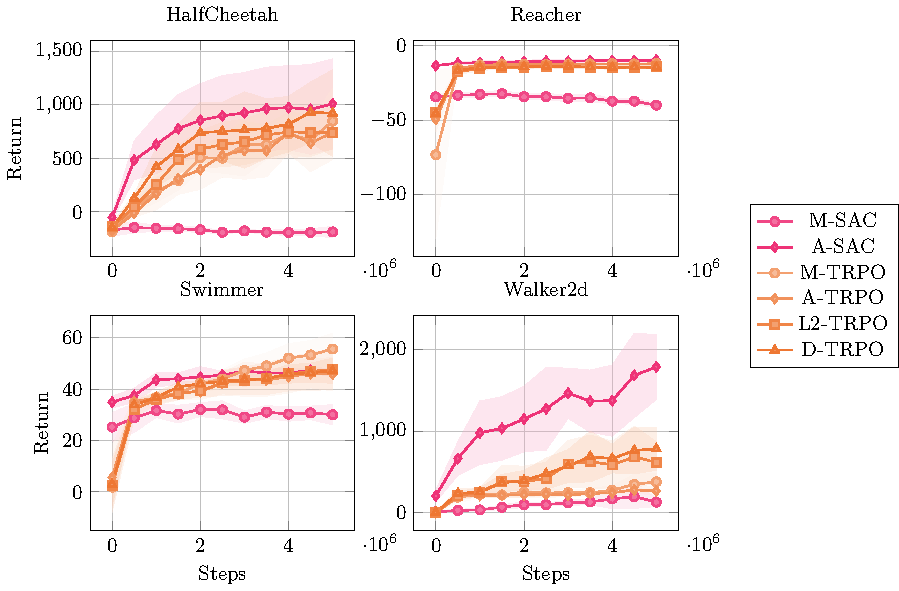
\includegraphics[labelbelief=dtrponetwork]{img/thesis_plots_belief.pdf}
    }
    \caption{D-TRPO 网络。从下至上：增广状态被拆分为序列 $(s,a_{i})_{i \in [\![1,\delay]\!]}$；序列经过一个 Transformer 编码器层，返回信念编码 $f_{\vectorialform{\phi}}(x)_i\in\realnumbers^{n_b}$；MAF 层以前一个编码向量为条件学习后续 $\delay$ 个状态的信念。最后，最后一个信念编码 $f_{\vectorialform{\phi}}(x)_\delay$ 用作策略的输入。}
    \label{fig:dtrpo_network}
\end{figure}


\begin{algorithm}[t]
\caption{信念表征网络训练}\label{algo:belief_training}
\textbf{Inputs}:
belief representation network parameters $\vectorialform{\phi}$ and $\vectorialform{\theta}$, number of epochs $K$, batch size $N$,number of samples $M$, empty replay buffer $\mathcal{D}$.\\
\textbf{Outputs}: Trained parameters $\vectorialform{\phi}$ and $\vectorialform{\theta}$.
\begin{algorithmic}[1]
    \FOR{$k=1,\dots,K$}%\{$1,\dots,N$\}}
        \STATE Collect $M$ samples under some policy $\pi$
        \STATE Add couples of augmented states $x=(s,a_1,\dots,a_{\delay})$ and corresponding sequence states to be predicted $(s_1,\dots,s_\delay)$ to $\mathcal{D}$
        \STATE Sample $N$ such couples from $\mathcal{D}$
        \STATE Update parameters $\vectorialform{\phi}$ and $\vectorialform{\theta}$ by descending the gradient $\nabla_{\vectorialform{\phi},\vectorialform{\theta}}\mathcal{L}_p$ (See \Cref{eq:loss_maf})
    \ENDFOR
\end{algorithmic}
\end{algorithm}

\subsection{同时学习多个延迟}
\label{subsec:multi_delay_once_belief}
本文提出一个简单思路，利用 D-TRPO 在给定整数延迟 $\delay>0$ 下学习的策略。
尽管思路简单，但先前文献未曾考虑过此想法。
本文提出通过模拟 $\delay$ 延迟，将 D-TRPO 应用于更小的整数延迟 $0<\delay'<\delay$。
具体而言，除了延迟 $\delay'$ 对应的增广状态 $x_t=(s_{t-\delay'},a_{t-\delay'},\dots,a_{t-1})$ 外，还考虑一个缓冲区，
\begin{align*}
    (s_{t-\delay},a_{t-\delay},\dots,s_{t-\delay'-1},a_{t-\delay'-1}),
\end{align*}
包含 $t-\delay'$ 之前最后 $\delay-\delay'$ 个状态和动作的历史记录。
通过这种方式，智能体可以构造一个合成增广状态 $x_t'=(s_{t-\delay},a_{t-\delay},\dots,a_{t-1})$。
这足以应用 D-TRPO 在延迟 $\delay$ 下学习的策略。
显然，该算法具有与延迟 $\delay$ 的 D-TRPO 相同的性能保证。
在\Cref{sec:exp_belief}中提供实验验证该思路的有效性。

对于文献中的某些方法，可以做得比上述简单思路更好。
例如，与\cite{firoiu2018human}类似，可以不学习信念表征，而是学习未来所有 $\delay$ 个状态的期望状态。
本文设计一种方法实现这一目标，使用与 D-TRPO 相同的网络结构，但移除 MAF 层。
网络训练以最小化其输出 $(f_\phi(\textbf{x})_i)_{i\in[\![1, d]\!]}$ 与真实状态 $(s_1,\dots,s_\delay)$ 之间的 L2 损失。
将其接入\gls{trpo}后，称该方法为 L2-TRPO。
在这种情况下，可以用另一种方式同时学习多个延迟。
事实上，因果 Transformer 网络的一个有趣特性是它可以被裁剪到所需长度，因此可以应用于更短延迟 $0<\delay'<\delay$ 的增广状态。
根据设计，L2-TRPO 也已学习未来 $\delay'$ 步的期望状态。
因此，裁剪后 Transformer 的输出可作为\gls{trpo}的输入。
值得注意的是，D-TRPO 无法做到这一点。尽管它学习了未来每个 $\delay$ 状态的信念表征，但各自的编码可能遵循不同规则。
因此，\gls{trpo}可能无法理解较早状态的编码。

此处提出的简单思路与\cite{chen2021delay}的论点一致：基于模型的方法更适合延迟场景，因为其模型可以复用。



\section{理论分析}
\label{sec:th_analysis_belief}

本节提供若干理论结果，帮助理解常值延迟\gls{dmdp}问题。
首先，本文形式化证明一个文献中通常视为理所当然的事实：延迟越长，最优回报越小。
第二部分研究常值延迟\gls{dmdp}的复杂度。
最后，通过一个示例证明基于模型的策略在某些问题中可能出现次优性能。


\subsection{延迟对性能的影响}
\label{subsec:effect_delay_belief}
对于平均奖励或期望折扣回报，在其他条件相同的情况下，\gls{dmdp}的延迟越大，其最优策略的性能越低，这似乎是合理的。
尽管直观自然，但该结果尚未得到证明。
下面给出证明。该结果需要以下假设，确保两个具有不同延迟的过程以相同方式初始化。

\begin{defi}[一致\glspl{dmdp}]
\label{def:consistency_dmdps}
     设 $\delayedmarkovdecisionprocess$ 和 $\delayedmarkovdecisionprocess'$ 为两个\glspl{dmdp}，其延迟分别为 $\delay$ 和 $\delay'$，初始增广状态分布分别为 $\delayeddiscountedstateoccupancydistribution[0][]$ 和 $\delayeddiscountedstateoccupancydistribution[0][\prime]$。
     若 $\delay\le \delay'$，则称 $\delayedmarkovdecisionprocess$ 和 $\delayedmarkovdecisionprocess'$ 是一致的，当且仅当：
    \begin{align*}
        \probability(S_0=s_0;\delayeddiscountedstateoccupancydistribution[0][])= \probability(S_0=s_0;\delayeddiscountedstateoccupancydistribution[0][\prime]),
    \end{align*}
    且 $\forall t\le\delay$，
    \begin{align*}
        \probability(A_t=a_t;\delayeddiscountedstateoccupancydistribution[0][])= \probability(A_t=a_t;\delayeddiscountedstateoccupancydistribution[0][\prime]).
    \end{align*}
\end{defi}


\begin{thm}
\label{th:perf_delay_vector_all_weight}
    设 $\delayedmarkovdecisionprocess_{1}$ 和 $\delayedmarkovdecisionprocess_{2}$ 为两个一致\glspl{dmdp}，其延迟分别为 $\delay_1$ 和 $\delay_2$。
    考虑 $\expectedreturn[1][\star]$ 和 $\expectedreturn[2][\star]$，分别为它们的最优期望折扣回报或平均奖励。
    若 $\delay_1<\delay_2$，则有：
    \begin{align*}
        \expectedreturn[2][\star] \le \expectedreturn[1][\star].
    \end{align*}
\end{thm}
\begin{proof}
    为证明该结果，首先证明 $\delayedmarkovdecisionprocess_{1}$ 中存在一个非平稳的基于历史的策略，其具有与 $\delayedmarkovdecisionprocess_{2}$ 中最优马尔可夫策略 $\optimalpolicy_2$ 相同的增广状态分布。
    为定义该策略，将轨迹分为两个时间段。
    在第一时间段，当 $t\ge\delay_2$ 时，记 $(s_{t-{\delay_2}},a_{\delay_2},\dots,s_{t-1},a_{t-1},s_t)$ 为最近 $\delay_2$ 步的历史。
    $\delayedmarkovdecisionprocess_{2}$ 中的智能体观测到增广状态
    \begin{align*}
        x_t'=(s_{t-{\delay_2}},a_{t-{\delay_2}},\dots,a_{t-1}).
    \end{align*}
    由于 $\delay_1<\delay_2$，$\delayedmarkovdecisionprocess_{1}$ 中的智能体可以观测到以下量
    \begin{align*}
        \overline x_t=(s_{t-{\delay_2}},a_{t-{\delay_2}},\dots,s_{t-{\delay_1}},a_{t-{\delay_1}}\dots,a_{t-1}),
    \end{align*}
    该量属于 $\statespace^{\delay_1-\delay_2}\times\actionspace^{\delay_2}$。
    注意，该"状态"包含 $\delay_1-\delay_2$ 个状态和动作的历史，这些在 $\delayedmarkovdecisionprocess_{1}$ 的马尔可夫策略中不会被使用。
    将候选策略 $(\pi_t)_{t\ge0}$ 对 $t\ge\delay_2$ 定义如下
    \begin{align*}
        \pi_t(\cdot\vert\overline x_t) = \optimalpolicy_2(\cdot\vert x_t').
    \end{align*}
    当 $\delay_1\le t<\delay_2$ 时，$\delayedmarkovdecisionprocess_{1}$ 中的智能体尚不能观测到 $\delay_2$ 步前的状态。
    然而，已知 $\delayedmarkovdecisionprocess_{2}$ 的初始状态分布 $\delayeddiscountedstateoccupancydistribution[0,2][]$，可以将策略定义为
    \begin{align*}
        \pi_t(a_t) = \probability(A_t=a_t;\delayeddiscountedstateoccupancydistribution[0,2][]).
    \end{align*}
    本质上，$\pi_t$ 忽略增广状态，以与 $\delayedmarkovdecisionprocess_{\delay_2}$ 中初始动作分布相同的概率选择动作。

    下面证明该策略在 $\delayedmarkovdecisionprocess_{2}$ 中诱导出相同的状态分布。
    记 $\delayeddiscountedstateoccupancydistribution[t][\pi]$ 为 $(\pi_t)_{t\ge0}$ 在时刻 $t$ 的未折扣状态分布，$\delayeddiscountedstateoccupancydistribution[t][\optimalpolicy_2]$ 为 $\optimalpolicy_2$ 的状态分布。
    对 $t=\delay_2$，注意到
    \begin{align}
        &\delayeddiscountedstateoccupancydistribution[t][\optimalpolicy_2](x_t')
        \nonumber\\
        &= \delayeddiscountedstateoccupancydistribution[0,2][](s_{t-{\delay_2}},a_{t-{\delay_2}},\dots,a_{t-1})
        \nonumber\\
        &= \delayeddiscountedstateoccupancydistribution[0,1][](s_{t-{\delay_2}},a_{t-{\delay_2}},\dots,a_{t+\delay_1-\delay_2-1})\prod_{i=1}^{\delay_2-\delay_1}\probability(A_{t-i}=a_{t-i};\delayeddiscountedstateoccupancydistribution[0,2][])
        \label{eq:consistency_dmdps}\\
        &=\delayeddiscountedstateoccupancydistribution[0,1][](s_{t-{\delay_2}},a_{t-{\delay_1}},\dots,a_{t+\delay_1-\delay_2-1})\prod_{i=1}^{\delay_2-\delay_1}\pi_{t-i}(a_{t-i})
        \label{eq:def_policy_less_delay}\\
        &\coloneq \delayeddiscountedstateoccupancydistribution[t][\pi](x_t'),\nonumber
    \end{align}
    其中 \Cref{eq:consistency_dmdps} 由一致性假设成立，\Cref{eq:def_policy_less_delay} 由 $(\pi_t)_{t\ge0}$ 在前 $\delay_2$ 步的定义成立。
    然后，假设对某个 $t\ge\delay_2$ 有 $\delayeddiscountedstateoccupancydistribution[t][\optimalpolicy_2]=\delayeddiscountedstateoccupancydistribution[t][\pi]$，证明对 $t+1$ 等式也成立。
    需要引入一些记号以简化表述。首先，对于 $\overline x_t,\overline x_{t+1}\in\statespace^{\delay_1-\delay_2}\times\actionspace^{\delay_2}$ 和 $a_t\in\actionspace$，记 $\bar{\transitionfunction}(\overline x_{t+1}\vert \overline x_t, a_t) = \probability(X_{t+1}=\overline x_{t+1}\vert X_t=\overline x_t,A_t=a_t)$ 为从 $(\overline x_t,a_t)$ 到 $\overline x_{t+1}$ 的转移概率。还定义以下测度，对 $x_t'\in\statespace\times\actionspace^{\delay_2}$
    \begin{align*}
        \delta_{x_{t}'}(\overline x_{t}) = \delta_{s_{t-\delay_2}'}(s_{t-\delay_2})\prod_{i=1}^{\delay_2}\delta_{a_{t-i}'}(a_{t-i}),
    \end{align*}
    这确保 $x_{t}'$ 中的状态和动作包含在 $\overline x_{t}$ 中。
    使用此记号，有
    \begin{align}
        \delayeddiscountedstateoccupancydistribution[t][\pi](x_{t+1}')
        &= \int_{\statespace^{\delay_1-\delay_2}\times\actionspace^{\delay_2}} \delayeddiscountedstateoccupancydistribution[t][\pi](\overline x_{t}) \bar{\transitionfunction}(\overline x_{t+1}\vert \overline x_t,a_t) \delta_{x_{t+1}'}(\overline x_{t+1})\pi_t(a_t\vert \overline x_t)\;\de \overline x_t\;\de s_{t-\delay_1+1}
        \nonumber\\
        &= \int_{\statespace^{\delay_1-\delay_2}\times\actionspace^{\delay_2}} \delayeddiscountedstateoccupancydistribution[t][\pi](\overline x_{t}) \bar{\transitionfunction}(\overline x_{t+1}\vert \overline x_t,a_t)
        \delta_{s_{t-\delay_2+1}'}(s_{t-\delay_2+1})\optimalpolicy_2(a_t\vert x_t')
        \nonumber\\
        &\qquad \prod_{i=0}^{\delay_2-1}\delta_{a_{t-i}'}(a_{t-i})\;\de\overline x_t\;\de s_{t-\delay_1+1}
        \nonumber\\
        &= \int_{\statespace^{\delay_1-\delay_2-1}\times\actionspace^{\delay_2+1}} \delayeddiscountedstateoccupancydistribution[t][\pi](\overline x_{t})  \delta_{s_{t-\delay_2+1}'}(s_{t-\delay_2+1})
        \optimalpolicy_2(a_t\vert x_t')
        \prod_{i=0}^{\delay_2-1}\delta_{a_{t-i}'}(a_{t-i})\;\de\overline x_t
        \label{eq:indpt_delta}
        \\
        &= \int_{\statespace\times\actionspace^{\delay_2}} \delayeddiscountedstateoccupancydistribution[t][\pi](x_{t}') p(s_{t-\delay_2+1}\vert s_{t-\delay_2},a_{t-\delay_2}) \delta_{s_{t-\delay_2+1}'}(s_{t-\delay_2+1})
       \nonumber
       \\
        &\qquad \cdot\optimalpolicy_2(a_t\vert x_t')\prod_{i=0}^{\delay_2-1}\delta_{a_{t-i}'}(a_{t-i})\;\de x_t'
        \label{eq:indpt_delta2}
        \\
        &= \int_{\statespace\times\actionspace^{\delay_2}} \delayeddiscountedstateoccupancydistribution[t][\optimalpolicy_2](x_{t}') \augmentedtransitionfunction(x_{t+1}'\vert x_t',a_t)\optimalpolicy_2(a_t\vert x_t')\;\de x_t'
       \nonumber
       \\
       &= \delayeddiscountedstateoccupancydistribution[t][\optimalpolicy_2](x_{t+1}'),\nonumber
    \end{align}
    其中 \Cref{eq:indpt_delta} 成立是因为 Dirac 测度 $\delta$ 涉及的所有项已由 $\overline x_t$ 和 $x_{t+1}'$ 固定，\Cref{eq:indpt_delta2} 成立是因为除 $\delayeddiscountedstateoccupancydistribution[t][\pi](\overline x_{t})$ 外没有项依赖于 $s_{t-\delay_2+2},\dots,s_{t-\delay_1}$，因此可以对这些项进行积分。

    综上所述，我们在 $\delayedmarkovdecisionprocess_{1}$ 中找到了一个非平稳的基于历史的策略，其在任意时刻具有与 $\delayedmarkovdecisionprocess_{2}$ 中最优策略相同的增广状态分布。
    根据设计，该策略在任何状态下选择与 $\optimalpolicy_2$ 相同的动作，因此在任何时刻获得相同的奖励。
    这表明 $(\pi_t)$ 和 $\optimalpolicy_2$ 具有相同的折扣期望回报或平均奖励。
    由于 $(\pi_t)$ 只是 $\delayedmarkovdecisionprocess_{1}$ 的一个特定策略，$\delayedmarkovdecisionprocess_{1}$ 中的最优策略可能产生更高的回报或平均奖励。证明完毕。
\end{proof}

\begin{remark}
    从\cite[Theorem~6.2.10 and Theorem~8.1.2]{puterman1994markov}我们甚至知道 $\delayedmarkovdecisionprocess_{1}$ 中存在一个最优马尔可夫策略（即仅使用增广状态而非更多历史），产生 $\expectedreturn[1][\star]$。
\end{remark}

通过一个推论扩展上述结果：尽管证明中设计的策略是基于历史的，但 $\delayedmarkovdecisionprocess_{1}$ 中存在一个马尔可夫策略（同样仅使用增广状态而非更多历史），其状态分布与 $\delayedmarkovdecisionprocess_{1}$ 中最优策略相同。

\begin{prop}
\label{corol:markov_optimal_delayed_equiv}
    设 $\delayedmarkovdecisionprocess_{1}$ 和 $\delayedmarkovdecisionprocess_{2}$ 为两个一致\glspl{dmdp}，其延迟向量分别为 $\delay_1$ 和 $\delay_2$，且 $\delay_1<\delay_2$。
    考虑 $\delayedmarkovdecisionprocess_{2}$ 中的一个马尔可夫策略 $\delayedpolicy_2$（即相对于其增广状态 $\augmentedstatespace_2=\statespace\times\actionspace^{\delay_2}$），具有 $\sigma$-有限占据测度。
    则 $\delayedmarkovdecisionprocess_{1}$ 中存在一个马尔可夫策略（相对于其增广状态 $\augmentedstatespace_1=\statespace\times\actionspace^{\delay_1}$），其在 $\augmentedstatespace_1$ 上诱导的状态-动作分布与最优策略 $\delayedpolicy_2$ 相同。
\end{prop}
\begin{proof}
    设 $\delayedpolicy_2$ 为 $\delayedmarkovdecisionprocess_{2}$ 中具有 $\sigma$-有限占据测度的策略。
    根据\Cref{th:perf_delay_vector_all_weight}的证明，可以在 $\delayedmarkovdecisionprocess_{1}$ 中构建一个基于历史的策略 $\delayedpolicy_1$，其在 $\augmentedstatespace_2$ 上具有相同的状态-动作分布。
    然后，根据\cite[Theorem~3]{laroche2022non}，$\delayedmarkovdecisionprocess_{1}$ 中存在一个马尔可夫策略 $\delayedpolicy$，其在 $\augmentedstatespace_1$ 上的状态分布与该 $\delayedpolicy_1$ 相同。
    证明完毕。
\end{proof}

\subsection{常值延迟的复杂度}
\label{subsec:delay_complexity}

以下命题直接源自\cite{bertsekas1987dynamic,altman1992closed}，该文献指出具有状态观测延迟和/或动作执行延迟的\gls{dmdp}可以通过增广状态转化为\gls{mdp}。
\begin{prop}
\label{pp:dmdp_pompd}
基于模型和无记忆方法将状态观测延迟或动作执行延迟的问题从\gls{dmdp}转化为\gls{pomdp}。
特别地，使用信念表征作为策略输入的框架可以归约为 POMDP。
\end{prop}
\begin{proof}
    从\cite{bertsekas1987dynamic,altman1992closed}可知，通过使用增广状态，\gls{dmdp}转化为\gls{mdp}。
    由于基于模型方法仅使用从增广状态计算的当前状态的某些统计量，而无记忆方法仅使用后者的部分信息，智能体策略所使用的观测可视为对真实增广状态的部分观测。
    这正是\gls{pomdp}的框架。
\end{proof}

这是一个负面结果，因为尽管 \gls{dmdp} 可以通过状态增广转化为 \gls{mdp}，但我们现在只处理其部分观测，而已知 \gls{pomdp} 比 \gls{mdp} 难解得多\cite[Theorem 6]{papadimitriou1987complexity}。
\cite[Theorem~2]{walsh2009learning}证实了这一点，他们指出使用增广状态在 \gls{dmdp} 中进行规划已经是 NP-Hard 问题。

\begin{figure}[t]
    \centering
    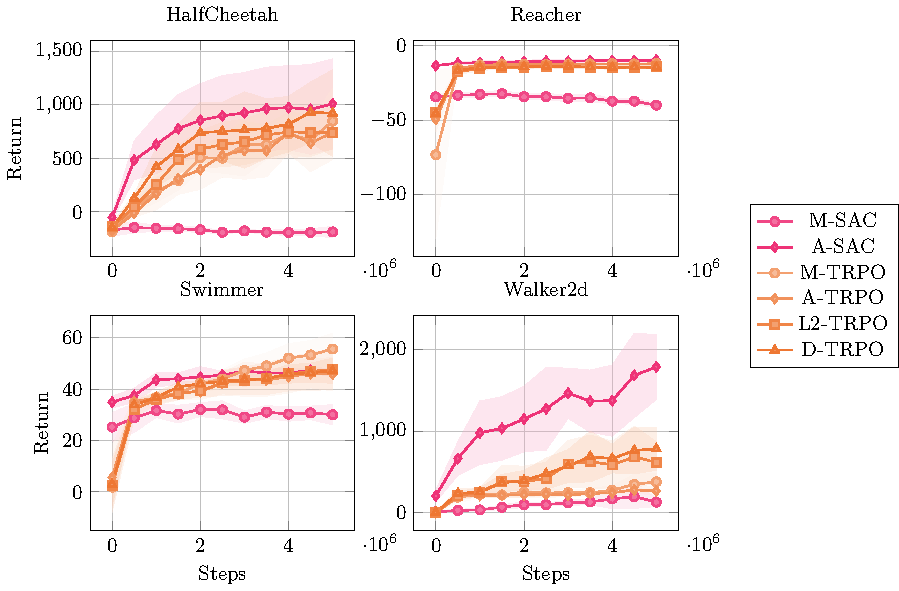
\includegraphics[labelbelief=mdppomdpsets]{img/thesis_plots_belief.pdf}
    \caption{相对于智能体可用信息量的问题维度。
    这些量之间的权衡由黑色虚线表示。
    无延迟\gls{mdp}（$\textbf{U}$）具有完全信息和低维度，而增广状态方法（$\textbf{A}$）是 MDP~\cite{bertsekas1987dynamic,altman1992closed}，具有更高维度。
    无记忆方法（$\textbf{Me}$）维度低，但如\Cref{pp:dmdp_pompd}所示属于\glspl{pomdp}。
    基于模型的方法（$\textbf{Mo}$）同样产生\glspl{pomdp}~\Cref{pp:dmdp_pompd}。
    后一种方法允许在维度和可观测性之间进行权衡。
    }
\label{fig:relations_dmdp_mdp_pomdp}
\end{figure}



\subsection{基于模型方法的反例}
\label{subsec:model_based_sub_optimal}

尽管上一节揭示了负面结果，但人们可能期望 \gls{dmdp} 的特殊结构允许基于模型的方法实现最优性能。
遗憾的是，以下命题证明基于模型策略集合上的最优回报相对于最优基于增广状态策略可能是次优的。

\begin{prop}
\label{pp:counter_example_belief_based}
    设 $\expectedreturn[b][*]$ 为同一 \gls{dmdp} 上基于信念的策略空间的最优回报，$\expectedreturn[a][*]$ 为基于增广状态的策略空间的最优回报。则存在 \glspl{dmdp} 使得
    \begin{align*}
        \expectedreturn[b][*]<\expectedreturn[a][*].
    \end{align*}
\end{prop}
\begin{proof}
    通过给出这样一个 \gls{dmdp} 的实例来证明。
    该实例在\Cref{fig:counter_example_dmdp_pomdp}中展示。
    在该实例中，延迟设为两步。智能体从最下方状态开始，为初始化过程，前两个动作均匀随机选择。在任何状态下，有两个可用动作 $a$ 和 $b$。
    注意，除最上方状态外，没有任何转移产生奖励。
    前者作为吸收态，提供节点上方标注的折扣回报或平均奖励。
    因此，智能体收集的奖励仅取决于其到达的最上方状态。
    除虚线标示的转移外，所有转移都是确定性的。
    在后一种情况下，沿任一路径前进的概率均为 $1/2$。
    该 \gls{mdp} 的特殊之处如下。
    由于两步延迟，初始化后智能体要么处于状态 $s$，要么处于状态 $s'$。
    这意味着，给定 \gls{mdp} 的结构，智能体对其当前状态的信念在 $s$ 和 $s'$ 上各为 $1/2$。
    值得注意的是，基于信念的策略无法区分智能体到达 $s$ 或 $s'$ 所经过的路径。
    第一条路径（红色）从初始状态确定性直接上移到下一个状态，然后转移到 $s$ 或 $s'$。
    第二条路径（蓝色）在第一步向左或向右，然后确定性转移到 $s$ 或 $s'$。
    蓝色路径的有趣特性在于，从第二步起，智能体将知道它会到达 $s$ 还是 $s'$。
    然而，在红色路径上，智能体需要多等待一步才能知道它实际处于 $s$ 还是 $s'$。
    基于信念的智能体无论沿哪条路径都看到相同的状态，而基于增广状态的智能体从增广状态中包含的第一个动作就能知道它将沿蓝色还是红色路径前进。
    因此，基于信念的智能体必须选择一条不考虑路径而优化回报的动作，而基于增广状态的策略可以利用这一额外信息更精细地选择动作。

    智能体需要选择后续两个动作才能获得最终奖励。
    对于红色路径，智能体在选择两个动作时不知道它将沿左分支还是右分支前进。
    智能体在各动作组合下获得的奖励见\Cref{tab:reward_red_path}。
    相反，对于蓝色路径，智能体可以根据其所沿 \gls{mdp} 分支调整第二个动作。
    类似地，\Cref{tab:reward_blue_path}给出了给定第一个动作和观测状态的奖励。
    注意，给定该状态和动作，下一步的最优动作是确定的。

    初始化设计使得智能体沿任一路径的概率相同。
    对于红色路径，智能体应先执行 $b$ 再执行 $a$，获得 $12.5$ 的奖励。
    对于蓝色路径，则应先选择动作 $a$，然后根据观测调整第二个动作，获得 $15$ 的平均奖励，而若先执行 $b$ 则仅获得 $12.5$ 的平均奖励。

    因此，基于增广状态的策略将遵循上述推理，平均获得 $\expectedreturn[a][*]=13.75$ 的奖励。
    基于信念的策略则被迫对两条路径首先选择相同的动作，因为它不知道将沿哪条路径前进。
    若先选择 $a$，智能体在红色路径情况下获得 $10$，在蓝色路径情况下获得 $15$。
    若先选择 $b$，则在红色路径情况下获得 $6.25$，在另一条路径上获得 $12.5$。
    这意味着，无论第一个动作如何选择，期望奖励总是更小。
    其最优回报通过先执行 $a$ 获得，为 $\expectedreturn[b][*]=12.5$。
    证明完毕。
\end{proof}


\begin{figure}[t]
    \centering
    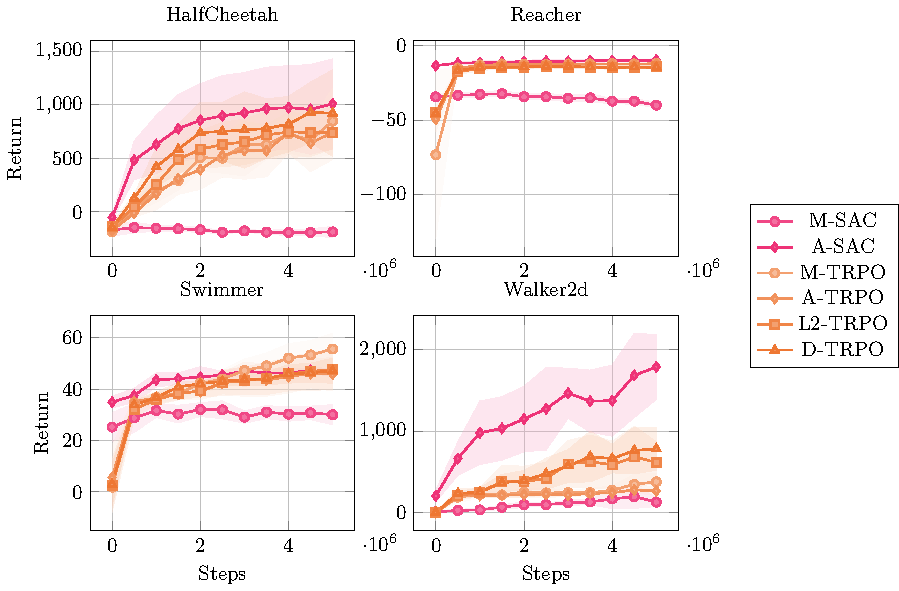
\includegraphics[labelbelief=counterexampledmdppomdp]{img/thesis_plots_belief.pdf}
    \caption{\gls{dmdp}实例，其中对于两步延迟，基于信念的策略相对于最优基于增广状态的策略是次优的。
    在任何状态下，智能体可以选择两个动作 $a$ 和 $b$ 之一。
    除最上方转移外，没有任何转移提供奖励。对于后者，一个循环状态提供节点上方标注的折扣回报或平均奖励。
    除虚线所示转移外，所有转移都是确定性的，其中选择给定动作的智能体各有 $1/2$ 的概率沿任一边前进。
    智能体从最下方状态开始。
    底层\gls{mdp}设计为具有两条路径，它们在状态 $s$ 和 $s'$ 上产生相同的信念。}
    \label{fig:counter_example_dmdp_pomdp}
\end{figure}


\begin{table}[t]
\centering
\begin{tabular}{l|rr}
  & \multicolumn{1}{c}{$a$} & \multicolumn{1}{c}{$b$} \\
\hline
$a$ & $5$ & $10$ \\
$b$ & $12.5$ & $0$ \\
\end{tabular}
\caption{\label{tab:reward_red_path}初始沿红色路径时，所有第一个（行）和第二个（列）动作组合的奖励。}
\end{table}

\begin{table}[t]
\centering
\begin{tabular}{l|rr}
  & \multicolumn{1}{c}{$s$} & \multicolumn{1}{c}{$s'$} \\
\hline
$a$ & $a\rightarrow10$ & $b\rightarrow20$ \\
$b$ & $a\rightarrow15$ & $a\rightarrow10$ \\
\end{tabular}
\caption{\label{tab:reward_blue_path}初始沿蓝色路径时，所有第一个动作（行）与下一步观测状态（列）组合的奖励。第二个动作最优选择并在表中标出。}
\end{table}

尽管这个反例令人沮丧，但本文在\Cref{sec:th_analysis_imitation}中对一种特殊类型的基于信念的策略进行了分析，并证明在光滑性条件下，该策略的回报与最优延迟策略的回报相差不超过一个常数。

\section{实验评估}
\label{sec:exp_belief}

本节评估信念表征网络在不同任务中的实证表现，包括确定性和随机环境。
在\Cref{subsec:setting_exp_belief}中描述每个任务、基线方法和 D-TRPO 的设定。
在\Cref{subsec:results_belief}中提供并讨论实验结果。

\subsection{设定}
\label{subsec:setting_exp_belief}

注意，所有基线、本文方法和所有任务的结果均在 10 个随机种子下取平均。

\subsubsection{任务}
\label{subsubsec:tasks}
\noindent\textbf{Pendulum.}\indent 在该任务中，智能体必须学习将钟摆向上旋转。
该任务是延迟\gls{rl}中的经典任务，因为传统\gls{rl}算法的性能随延迟增大而迅速下降。
部分原因在于上方位置的不稳定平衡点，在延迟情况下难以维持。
在实现中，使用 \texttt{gym} 库~\cite{brockman2016gym}的版本。
该环境是确定性的。
鉴于在 Pendulum 上运行实验的计算成本相对较低，我们对集合 $\{3, 5, 10, 15, 20\}$ 中的常值延迟重复分析。
对该任务，执行 500 轮（epoch），每轮 5,000 步，总计 250 万步。

\noindent\textbf{随机 Pendulum.}\indent 该任务与前一个任务相同，但人为地向过程添加随机性。
具体而言，向智能体选择的动作添加形式为 $\epsilon = \text{scale}( \eta+ \text{shift})$ 的独立同分布噪声，其中 $\eta$ 为某个概率分布。
\Cref{tab:noises}给出了考虑的六种噪声。
还考虑一种额外噪声：环境以 0.9 的概率遵循智能体指示的动作，否则均匀随机采样一个动作。
将此过程称为\emph{均匀}（uniform）噪声。
对这些任务，仅考虑延迟为 5，执行 1,000 轮，每轮 5,000 步，总计 500 万步。

\begin{table}[t]
\centering
    \begin{tabular}{|l||l|l|l|l|}
        \hline
        Noise & Distribution  $\eta$ & Shift & Scale & Group \\ \hline
        \textit{Beta (8,2)}& $\beta (8,2)$ & $0.5$ & $2$ &  1\\
        \textit{Beta (2,2)} & $\beta (2,2)$ & $0.5$ & $2$ & 1\\
        \textit{U-Shaped} & $\beta (0.5,0.5)$ & $0.5$ & $2$ & 1\\
        \textit{Triangular} & $\text{Triangular} (-2,1,2)$ & $0$ & $1$ & 2\\
        % \textit{Uniform} & $\text{U} (-1,1)$ & $0$ & $1$ & 2\\
        \textit{Lognormal (1)} & $\text{Lognormal} (0,1)$ & $-1$ & $1$ & 3\\
        \textit{Lognormal (0.1)} & $\text{Lognormal} (0,0.1)$ & $-1$ & $1$ & 3\\
        \hline
    \end{tabular}
    \caption{随机 Pendulum 中动作添加噪声的分布。}
    \label{tab:noises}
\end{table}

\noindent\textbf{Mujoco.}\indent 这是一个连续机器人运动控制任务，使用 \texttt{mujoco}~\cite{todorov2012mujoco} 库提供的高级物理模拟器。
这些任务的复杂性在于其复杂的动力学以及大状态和动作空间。
从所有 Mujoco 环境中，考虑 Walker2d、HalfCheetah、Reacher 和 Swimmer，这些环境在早期测试后证明受延迟影响最大。
与 Pendulum 类似，这可以用某些情况下存在不稳定平衡点来解释。
这些环境是确定性的。
对这些任务，仅考虑延迟为 5，执行 1,000 轮，每轮 5,000 步，总计 500 万步。


\subsubsection{基线方法}
\label{subsubsec:baselines}
作为基线，包括基于增广状态的 \gls{trpo}（A-TRPO）和无记忆 \gls{trpo}（M-TRPO），以覆盖基于 \gls{trpo} 的方法谱系。
此外，考虑 \gls{sac}，因其在延迟应用中取得了优异的实证结果\cite{ramstedt2019real,bouteiller2020reinforcement}。
还在基线中包括基于增广状态的 \gls{sac}（A-SAC）和无记忆 \gls{sac}（M-SAC）。
\gls{sac} 的一个超参数是其更新频率。
尽管将该参数设置为每一步都重新训练可提高样本效率，但会显著增加计算时间和内存占用。
因此，仅在 Pendulum 上每一步都训练 \gls{sac}，而在 Mujoco 上限制为每 50 步训练一次以加速过程。
曾考虑加入 DCAC~\cite{bouteiller2020reinforcement}，但其实现计算开销较大，决定不纳入。
早期实验结果表明其运行时间超过其他算法的 10 倍以上。
此外，考虑 SARSA 和 $\lambda=0.9$ 的 dSARSA，但仅用于 Pendulum 环境。由于 SARSA 是一种批量\gls{rl}算法，需要对状态和动作空间进行仔细离散化，这直接影响最终性能。
因此，需要额外的离散化验证步骤。
对 Pendulum，使用经过调优的 15x15 状态空间网格和总共五个离散动作。
最后，在测试中将 L2-TRPO 作为基线，该方法采用与\cite{firoiu2018human}类似的方法学习状态的期望值。


\subsubsection{D-TRPO 的设定}
在呈现的实验中，测试 D-TRPO，即信念表征网络接入\gls{trpo}~\cite{schulman2015trust}后的结果。
一个重要说明是，经过 D-TRPO 的早期实验，我们注意到信念模块优化过程中信念表征可能发生显著变化。
这反过来导致 \gls{trpo} 策略优化不稳定，因为其输入分布不断变化。
为缓解此问题，在 200 轮后提前停止信念表征模块的训练。


\subsection{结果}
\label{subsec:results_belief}

\begin{figure}[t]
    \centering
    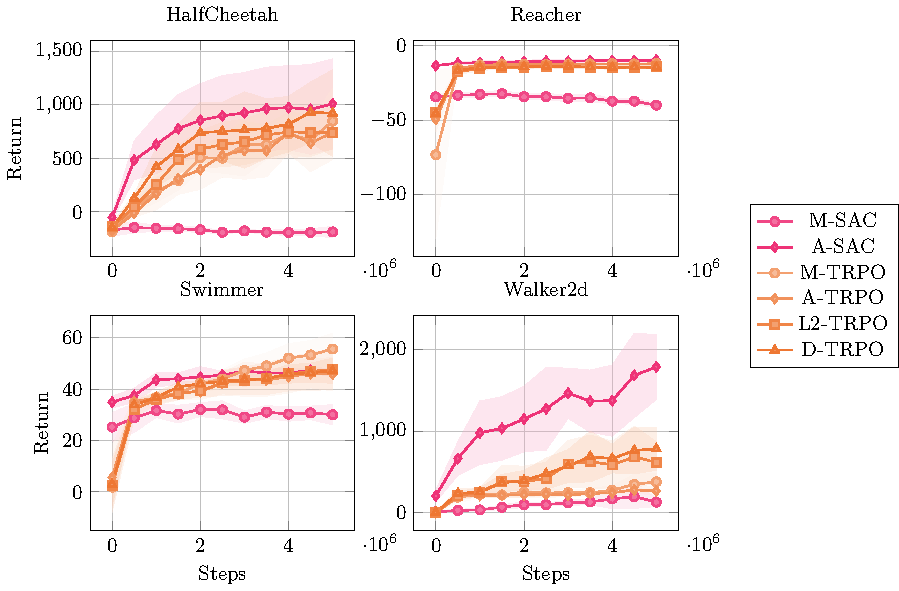
\includegraphics[labelbelief=pendulumvaryingdelay]{img/thesis_plots_belief.pdf}
    \caption{Pendulum 环境中 D-TRPO 和基线方法在不同延迟值下的平均回报。
    水平虚线表示无延迟 \gls{sac} 的性能。
    阴影区域表示一个标准差，结果基于 10 个随机种子获得。}
    \label{fig:pendulum_varying_delay_belief}
\end{figure}

\noindent\textbf{Pendulum.}\indent 不同方法和不同延迟值下的回报见\Cref{fig:pendulum_varying_delay_imitation}。
水平虚线表示无延迟版本 \gls{sac} 获得的回报。
对于不超过五的延迟，D-TRPO 和 L2-TRPO 的回报与无延迟 \gls{sac} 相当。
同时注意 A-SAC 在此情况下的优异表现。
然而，随着延迟增加，D-TRPO 和 L2-TRPO 的性能下降比 A-SAC 更显著。
在\Cref{fig:delay_5_pendulum_belief}中，聚焦延迟为 5 时 D-TRPO 和基线方法在学习阶段的表现。
图中还报告了无延迟 \gls{trpo} 的结果。自然，后者比任何基于 \gls{trpo} 的延迟方法更快，但有趣的是，它比 A-SAC 慢。
这表明 SAC 在解决此问题时特别有效，即便存在延迟。
除 A-SAC 外，D-TRPO 和 L2-TRPO 具有最快的收敛速度，与无延迟 TRPO 相比，需要额外约 100 万步才能达到类似策略。



\begin{figure}[t]
    \centering
    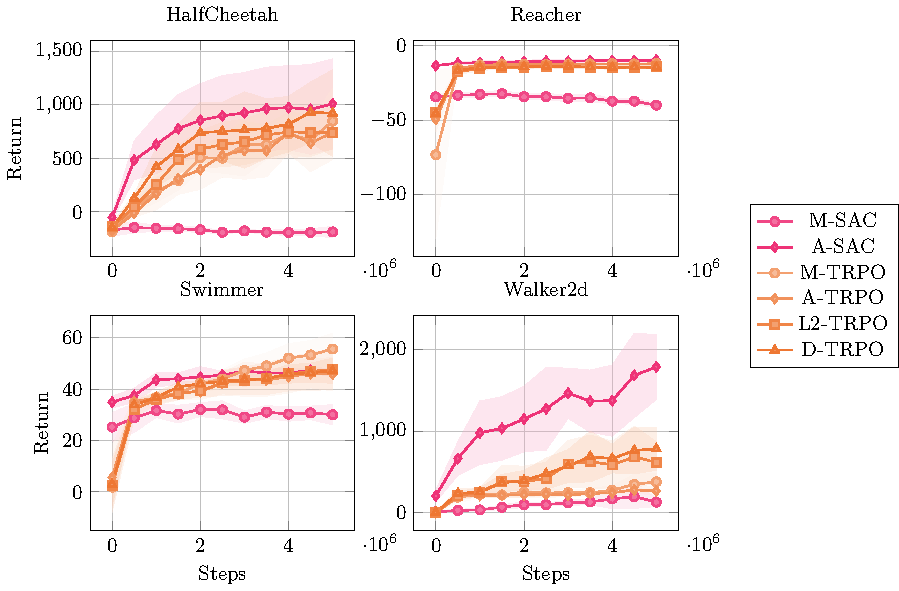
\includegraphics[labelbelief=delay5pendulumbelief]{img/thesis_plots_belief.pdf}
    \caption{D-TRPO 和 L2-TRPO 与延迟为 5 的 Pendulum 任务中其他基线方法的回报比较。包含无延迟 \gls{trpo} 的性能（记为``TRPO'')作为对照。
    阴影区域表示一个标准差，结果基于 10 个随机种子获得。}
    \label{fig:delay_5_pendulum_belief}
\end{figure}

\noindent\textbf{Mujoco.}\indent 在\Cref{fig:delay_5_mujoco_belief}中，报告 Mujoco 环境的结果。
此处同样，A-SAC 特别高效，仅在 Swimmer 环境中未获第一。
令人惊讶的是，在 500 万步后，M-TRPO 在该环境中表现最佳。
D-TRPO 和 L2-TRPO 在所有环境中表现良好，仅在 Walker2d 上出现明显性能不足。

\begin{figure}[t]
    \centering
    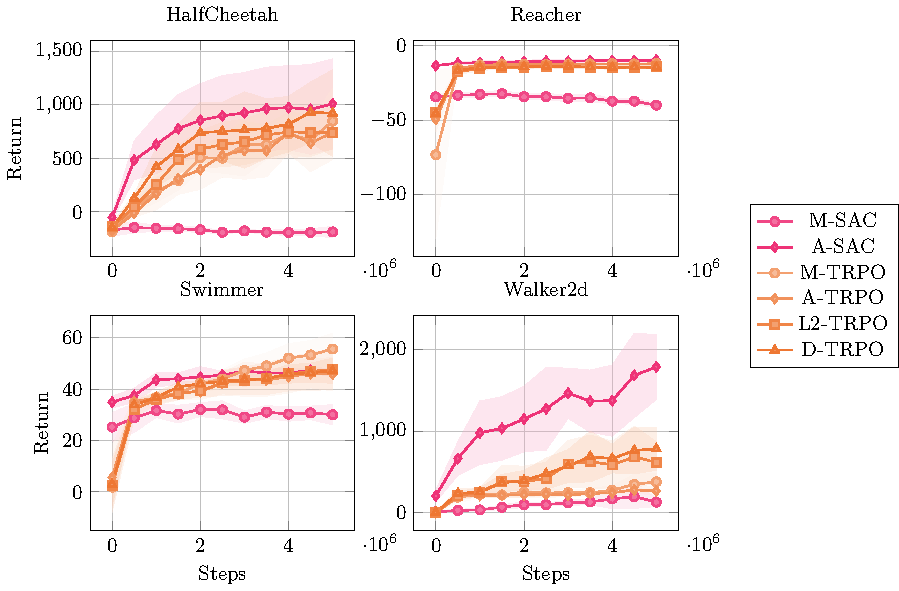
\includegraphics[labelbelief=delayfivemujocobelief]{img/thesis_plots_belief.pdf}
    \caption{D-TRPO 和 L2-TRPO 与基线方法在各种 Mujoco 环境中的回报比较。
    阴影区域表示一个标准差，结果基于 10 个随机种子获得。}
    \label{fig:delay_5_mujoco_belief}
\end{figure}

\noindent\textbf{随机 Pendulum.}\indent 在该任务上，仅比较 D-TRPO 与 L2-TRPO，以评估学习未来状态信念表征相对于其均值的优势。
结果报告在\Cref{fig:delay_5_pendulum_noise_belief}中。
为便于阅读结果，将噪声分为三组。
可以观察到 D-TRPO 从未被 L2-TRPO 超越。
对于某些噪声类型，如 Uniform 和 Triangular 噪声，两者获得相似的性能。
然而，对于其他类型的噪声，如 Quadratic 和 LogNormal (0.1) 情况，性能差异更为明显。
这表明信念表征在最坏情况下并非必要，但在最佳情况下可提供更高性能。

\begin{figure}[t]
    \centering
    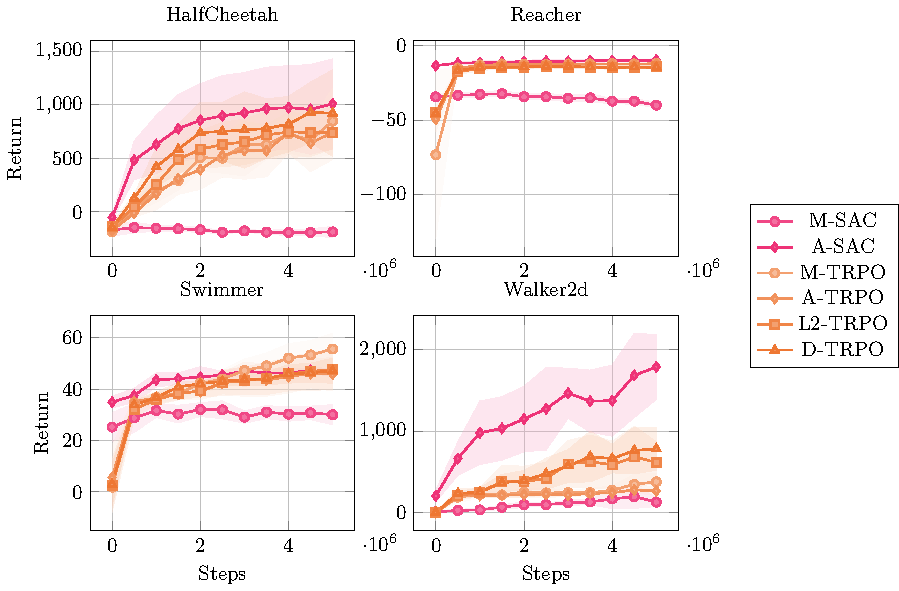
\includegraphics[labelbelief=pendulumnoisebelief]{img/thesis_plots_belief.pdf}
    \caption{D-TRPO 和 L2-TRPO 与基线方法在添加不同噪声（如\Cref{tab:noises}所述）的 Pendulum 环境中的回报比较。
    颜色表示噪声类型，标记表示算法。
    阴影区域表示一个标准差，结果基于 10 个随机种子获得。}
    \label{fig:delay_5_pendulum_noise_belief}
\end{figure}


\noindent\textbf{同时学习多个延迟.}\indent
\label{subsec:learning_multi_delay_once_belief}
在该实验中，测试\Cref{subsec:multi_delay_once_belief}中提出的思路，即 D-TRPO 和 L2-TRPO 在某个延迟 $\delay>0$ 下学习的策略应用于另一个延迟 $0<\delay'<\delay$。
在\Cref{fig:multi_delay_pendulum_dtrpo}中，提供 Pendulum 任务上 D-TRPO 和 L2-TRPO 以 $\delay=5$ 训练的结果。
在\Cref{fig:multi_delay_mujoco_dtrpo}和\Cref{fig:multi_delay_mujoco_ltrpo}中，提供 Mujoco 任务上 D-TRPO 和 L2-TRPO 以 $\delay=5$ 训练的结果。
显然且符合预期，较小延迟下获得的性能与原始性能相当。

\begin{figure}[t]
    \centering    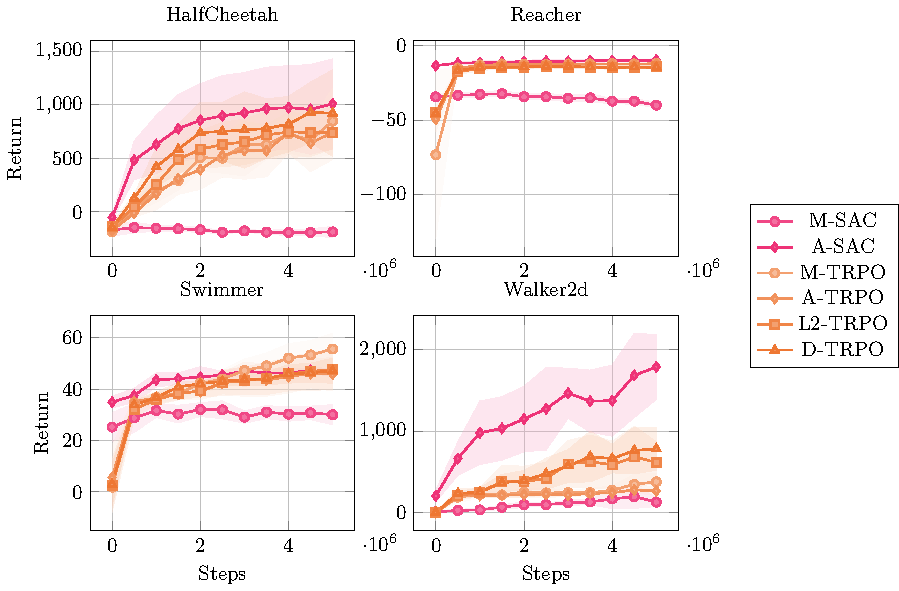
\includegraphics[labelbelief=multipledelayspendulumdtrpo]{img/thesis_plots_belief.pdf}
    \caption{延迟 10 训练的 D-TRPO 在 Pendulum 上以更小延迟测试的回报。}
    \label{fig:multi_delay_pendulum_dtrpo}
\end{figure}

\begin{figure}[t]
    \centering
    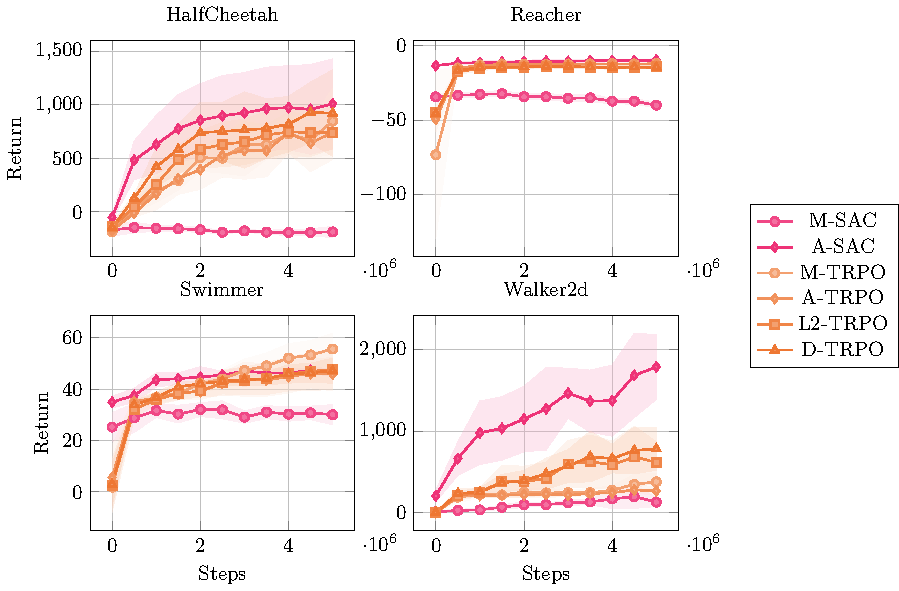
\includegraphics[labelbelief=multipledelaysmujocodtrpo]{img/thesis_plots_belief.pdf}
    \caption{延迟 5 训练的 D-TRPO 在 Mujoco 环境中以更小延迟测试的回报。}
    \label{fig:multi_delay_mujoco_dtrpo}
\end{figure}

\begin{figure}[t]
    \centering
    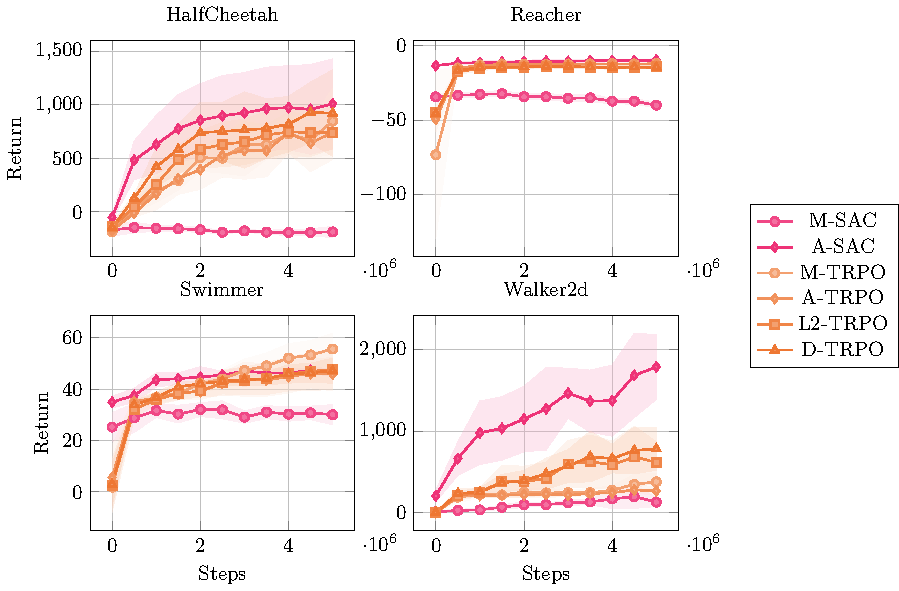
\includegraphics[labelbelief=multipledelaysmujocoltwotrpo]{img/thesis_plots_belief.pdf}
    \caption{延迟 5 训练的 L2-TRPO 在 Mujoco 环境中以更小延迟测试的回报。}
    \label{fig:multi_delay_mujoco_ltrpo}
\end{figure}

\section{结论}

本章针对常值延迟问题提出了一种基于模型的方法。
核心思想是学习信念的向量表征，将无限维量转化为有限维。
这得益于对\gls{nn}的精心选择。
该信念表征可作为状态的预处理模块接入任何\gls{rl}算法，正如本文将其接入\gls{trpo}构建 D-TRPO 一样。
通过一个简单技巧，展示了如何利用 D-TRPO 在较大延迟下学习的策略，直接应用于更小延迟。
该技巧显著降低了适应延迟的学习成本，因为可以同时学习多个延迟。
实验评估证实了这一可预见的结果，策略在任何更小延迟下均取得相似的性能。

随后对常值延迟问题进行了分析。
延迟越长、最优性能越低这一事实已得到形式化证明，该证明可为未来分析提供有用工具。
此外，揭示了基于模型方法的复杂度结果，展示了该方法的局限性。
基于相同思路，给出了一个反例，证明与最优延迟策略相比，基于模型的策略在某些\glspl{mdp}中可能产生次优的期望回报或平均奖励。

最后，通过实验分析评估了 D-TRPO 的能力。
实验表明，尽管 A-SAC 是整体上最有效的方法，但 D-TRPO 能够适应广泛场景，特别是随机\glspl{mdp}，甚至也包括确定性环境。
因此，信念表征网络是一种通用方法，可作为任何\gls{rl}算法的即插即用预处理模块。
值得注意的是，它允许控制信念表征的大小，从而控制\gls{rl}算法输入的维度。

一个有价值的未来方向是利用模型的知识将其融入\gls{rl}算法内部，例如增强演员-评论家方法中的评论家更新。

